\documentclass[11pt, a4paper, oneside]{article}

% URLs and hyperlinks ---------------------------------------
\usepackage{hyperref}
\hypersetup{
	colorlinks=true,
	linkcolor=blue,
	filecolor=magenta,      
	urlcolor=blue,
}
\usepackage[inline]{enumitem}
\usepackage{xurl}

% code snippet -------------------------------------------------------
\usepackage{minted}
% ---------------------------------------------------------------------

% page headers -------------------------------------------------
\usepackage{fancyhdr}
\fancypagestyle{plain}{\fancyhf{}\renewcommand{\headrulewidth}{0pt}}
\pagestyle{fancy}
\fancyhf{}
\fancyhead[L]{\nouppercase\leftmark}
\fancyhead[R]{\thepage}

% adjust a verrrrry big table -------------------------------
\usepackage{adjustbox}

% titlepage -------------------------------------------------
\usepackage{pdfpages}
\usepackage{svg}

% captions -------------------------------------------------
\usepackage[font=small,labelfont=bf]{caption}

% multiple figures ------------------------------------------
\usepackage{graphicx,subcaption}

% custom enumeration -----------------------------------------
\newcounter{itemadded}
\setcounter{itemadded}{0}
\newcommand{\addeditem}{%
	\addtocounter{enumi}{-1}%
	\stepcounter{itemadded}
	\let\LaTeXStandardLabelEnumi\labelenumi%
	\addtocounter{enumi}{1}
	\renewcommand{\labelenumi}{\arabic{enumi}\lr{R}.}%
	\item 
	\let\labelenumi\LaTeXStandardLabelEnumi%
}

\let\LaTeXStandardEnumerateBegin\enumerate
\let\LaTeXStandardEnumerateEnd\endenumerate

\renewenvironment{enumerate}{%
	\LaTeXStandardEnumerateBegin%
	\setcounter{itemadded}{0}
}{%
	\LaTeXStandardEnumerateEnd%
}

% tables -------------------------------------------------------
\usepackage{float}
\usepackage{multirow}
\renewcommand{\arraystretch}{1.23}

% Persian configuration ---------------------------------------
\usepackage{xepersian}
\settextfont{Yas}
\setdigitfont{Yas}
\setlatintextfont{Liberation Serif} % Use a dedicated Latin font for better spacing

% Line spacing adjustment -------------------------------------
\usepackage{setspace}
\linespread{1.5} % Adjust overall line spacing (1.0 for normal, 1.5 for increased)

\begin{document}
	
	\begin{titlepage}
		\centering
		\includesvg[width=3.8cm]{./layout/besm}\par
	
		\vspace{1cm}
    \includesvg[width=3.2cm]{./layout/logo}\par % Do not include the .svg extension
		
		\vspace{1mm}
		{\LARGE دانشگاه اصفهان}\par
		\vspace{1mm}
		{\Large دانشکده مهندسی کامپیوتر}\par
		
		\vspace{2cm}
		
		{\Large فاز سوم پروژه در مبانی هوش و کاربردها}\par
		\vspace{1cm}
		{\Huge جستجو در بازی‌ها}\par
		
		
		\vspace{2cm}
		{\Large استاد درس: دکتر حسین کارشناس}\par
		\vspace{0.5cm}
		{\Large دستیار استاد: پوریا صامتی}
		
		\vspace{1cm}
		{\Large دانیال شفیعی}\par
		{\Large مهدی مهدیه}\par
		{\Large سید امیررضا نجفی}\par
		
		\vspace{1.5cm}
		
		% Bottom of the page
		{\large دی ۱۴۰۳\par}
	\end{titlepage}
	\tableofcontents
	\newpage

	
		\section{بخش اصلی}
		
		
		
		
		
		\subsection{مقدمه}
در بخش اول پروژه، از الگوریتم minimax استفاده شده است. در الگوریتم پیاده‌سازی شده، الگوریتم تا عمق هفتم پیشروی می‌کند و شاخه‌هایی را که به سود بازیکن ماکس یعنی مرغ نیست را با روش هرس آلفا و بتا حذف می‌کند تا فرایند پیشروی در درخت بازی با سرعت بیشتری طی شود و بتوان در عمق بیشتری پیشروی کرد. این به این معنی است که ابتدا یک حرکت بازیکن ماکس که مرغ است می‌زند بعد نوبت به بازیکن حریف که ملکه است می‌رسد دوباره نوبت به بازیکن مرغ می‌رسد این فرایند مرحله‌به‌مرحله تا عمق ۷ پیش می‌رود. حرکت مرغ یک عمق و حرکت ملکه نیز یک عمق جدا محسوب می‌شود.

علاوه بر محیط‌های بازی شامل محیط simple و hard برای بهتر کارکردن الگوریتم و صحت سنجی عملکرد خوب تابع اکتشافی یک سری محیط خودساز ایجاد شده است که عملکرد را بتوان بهتر کرد.
محیط‌های خودساز که شرایط پیچیده‌تری از دو محیط پروژه دارند شامل ۹ محیط به نام‌های
\lr{ test1}
 تا
 \lr{test9}
   است.
   
   \begin{figure}[H]
   	\begin{subfigure}{0.35\textwidth}
   		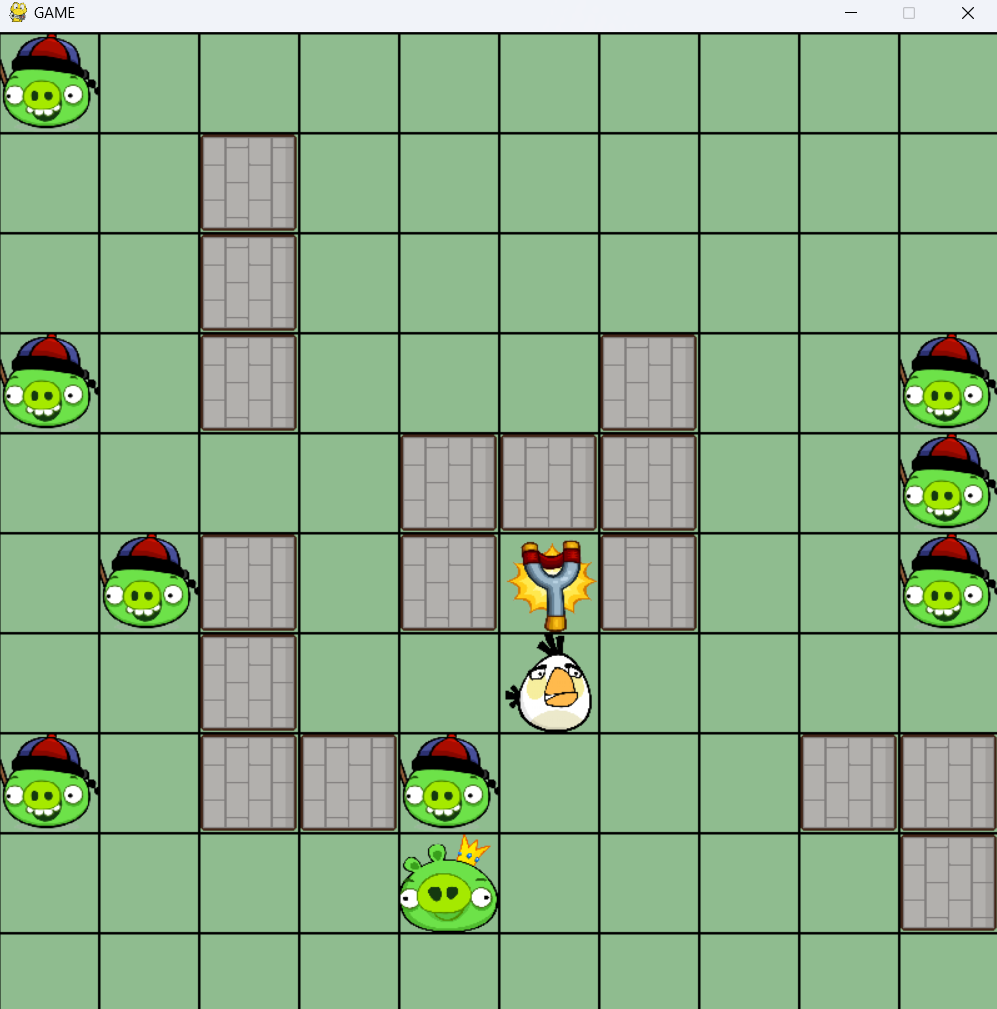
\includegraphics[width=\textwidth]{./images/game_simple}
   		\caption{محیط بازی ساده در انتها}
   		\label{fig:a}
   	\end{subfigure}
   	\hfill
   	\begin{subfigure}{0.35\textwidth}
   		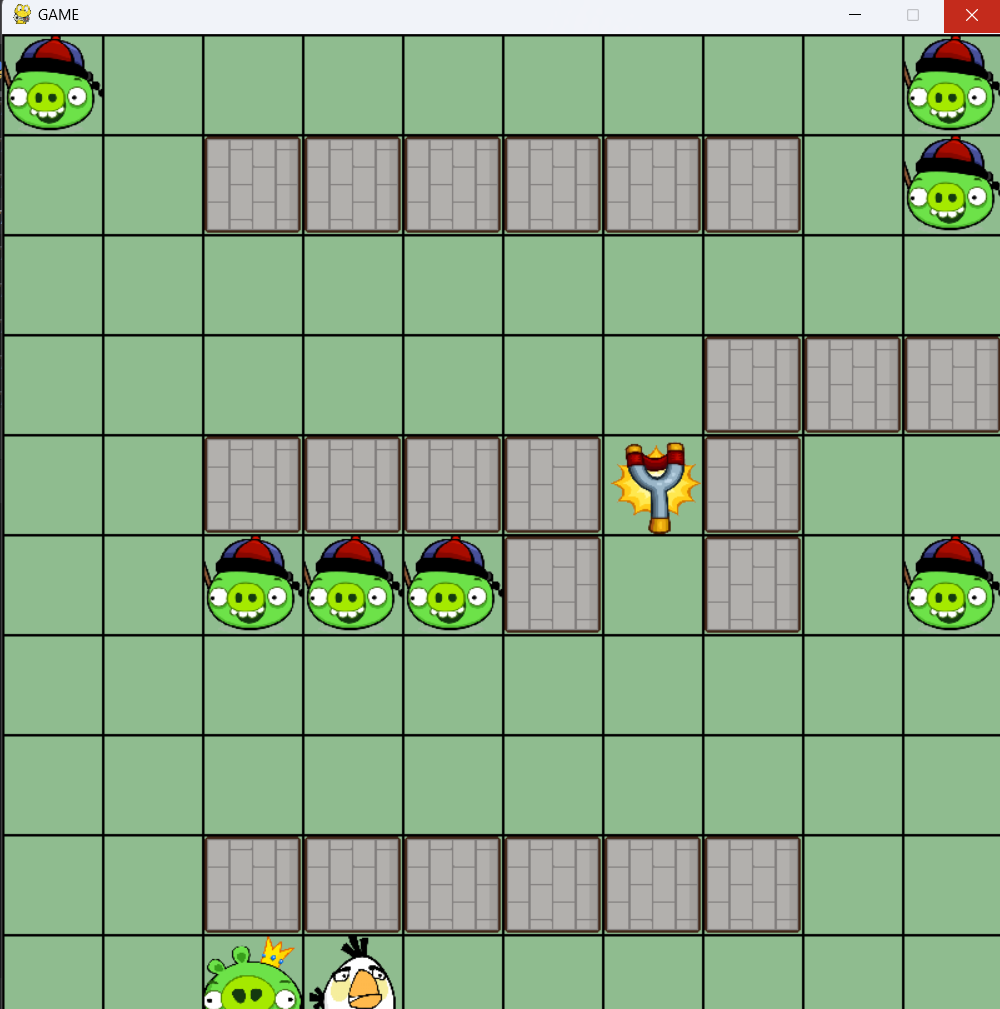
\includegraphics[width=\textwidth]{./images/game_hard}
   		\caption{محیط بازی سخت در انتها}
   		\label{fig:b}
   	\end{subfigure}
   	
   	\medskip
   	\begin{subfigure}{0.35\textwidth}
   		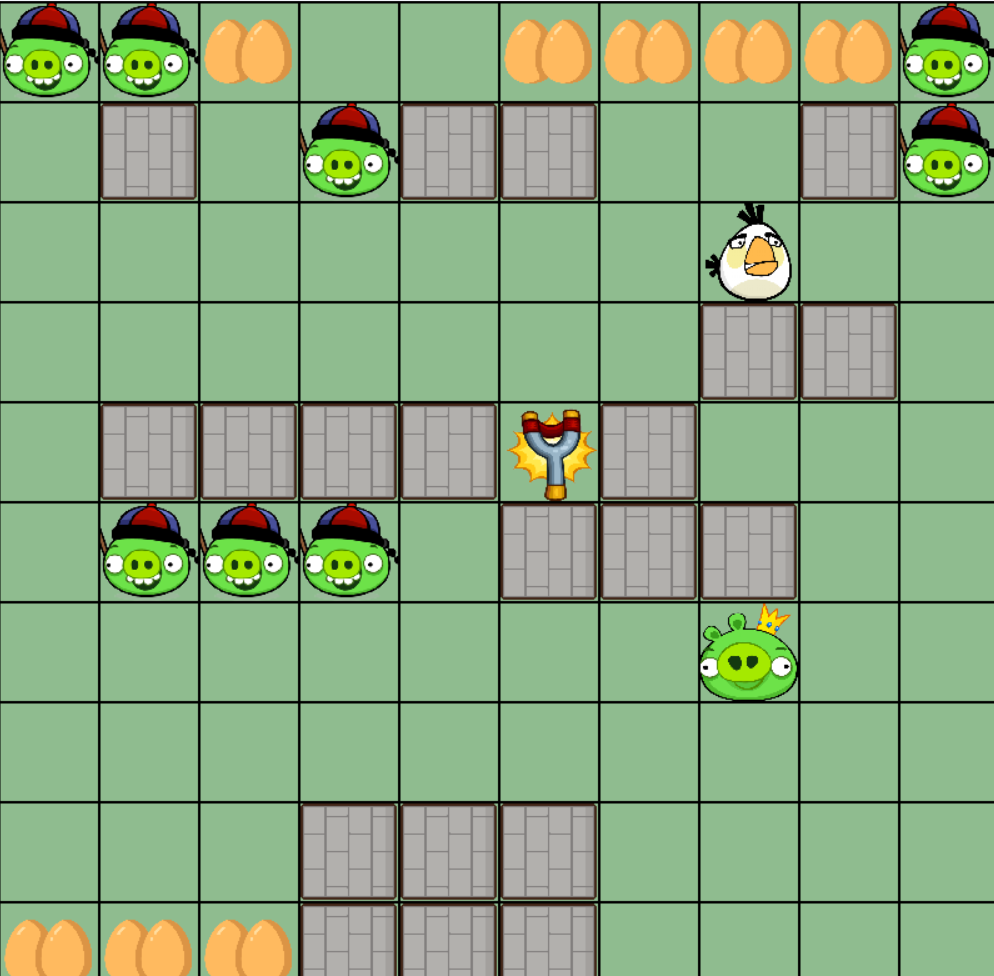
\includegraphics[width=\textwidth]{./images/game_t1}
   		\caption{محیط بازی تست ۱ در ابتدا}
   		\label{fig:c}
   	\end{subfigure}
   	\hfill
   	\begin{subfigure}{0.35\textwidth}
   		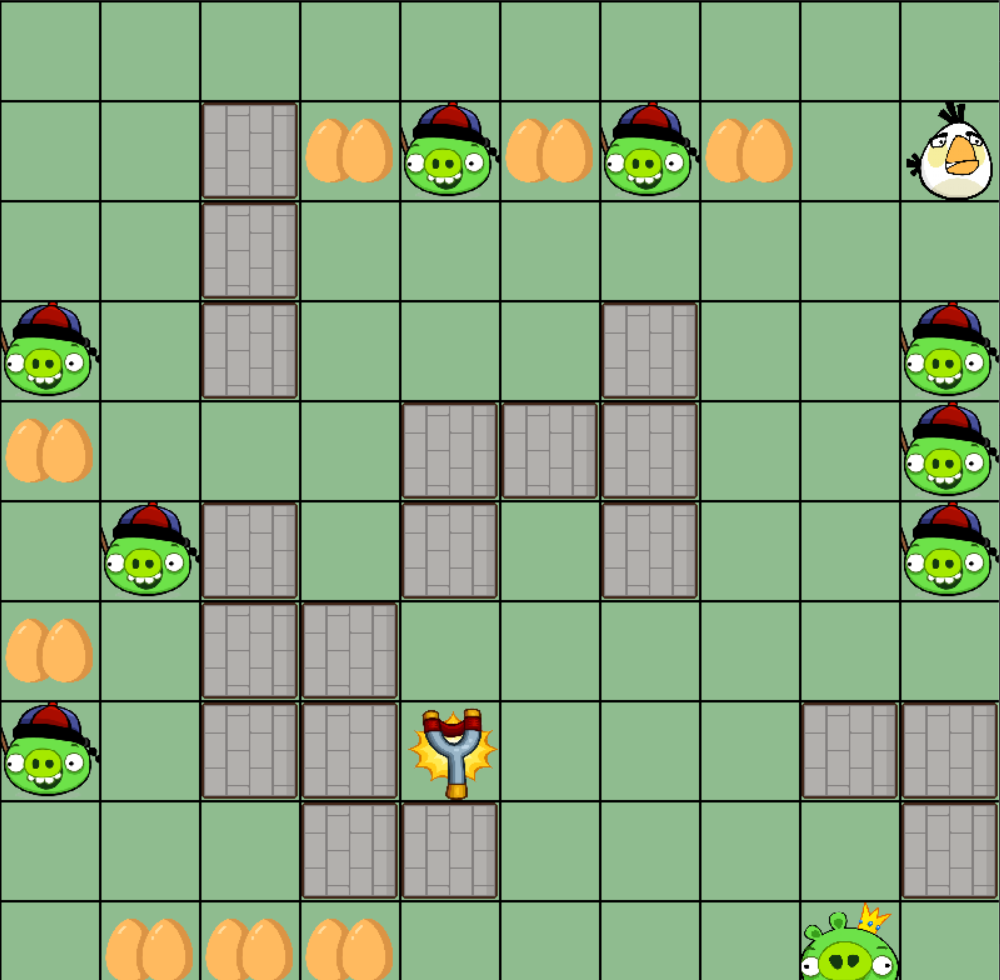
\includegraphics[width=\textwidth]{./images/game_t5}
   		\caption{محیط بازی تست ۵ در ابتدا}
   		\label{fig:d}
   	\end{subfigure}
   	
   	\caption{محیط‌های بازی در نقطه‌ی پایان و محیط تست در نقطه‌ی شروع}
   	\label{grids}
   	
   \end{figure}
   
\subsection{پیاده‌سازی الگوریتم مینی‌ماکس}
در تابع اکتشافی بعضی از فاصله‌ها به‌جای اندازه‌گیری اقلیدسی، با استفاده از دو الگوریتم bfs و ucs  به دست آورده شده‌اند به طور مثال فاصله واقعی مرغ تا تخم‌مرغ‌ها و فاصله مرغ تا پرتابگر.
فاصله مرغ تا ملکه به‌صورت اقلیدسی محاسبه می‌شود به دلیل عملکرد بهتر مرغ نسبت به سایر روش‌های محاسبه فاصله.

تابع اکتشافی بدین صورت عمل می‌کند که درصورتی‌که امتیازی که تا الان به دست آورده شده است (base\_score) از ۱۲۰۰ امتیاز بیشتر بود یا مجموع تعداد کنش‌های مرغ تابه‌حال (num\_actions) و فاصله تا پرتابگر بیشتر از ۱۴۰ بود (این به این معنی است که به اواخر بازی و امتیازی که مورد انتظار است نزدیک‌تر شده است) 
بررسی می‌کند که درصورتی‌که مرغ به پرتابگر نرسیده باشد امتیاز تابع اکتشافی می‌شود تفریق بین امتیازهای به دست آورده شده تابه‌حال (base\_score) و فاصله مرغ تا پرتابگر (sling\_dist) 
اما درصورتی‌که مرغ به پرتابگر رسیده باشد اگر امتیاز محاسبه شده تا کنون بالای ۱۵۰۰ باشد به این معنی است که مرغ عملکرد خوبی داشته است و همان بازگشت داده می‌شود به‌عنوان امتیاز تابع اکتشافی و اما اگر امتیاز بالای ۱۵۰۰ نبود یک امتیاز ۴۰۰ منفی در نظر گرفته می‌شود؛ زیرا با این که پرتابگر خورده شده و بازی به پایان رسیده است؛ اما برای رسیدن به پرتابگر زمان سریعی بوده است و مرغ امتیاز مورد انتظار را نتوانسته است به دست بیاورد. لازم به ذکر است امتیاز مورد انتظار در این پروژه امتیازی بالاتر از ۱۶۰۰ محسوب می‌شود.

درصورتی‌که شرط بیشتر بودن امتیاز به دست آورده شده تابه‌حال بیشتر از ۱۲۰۰ باشد و یا ادامه شرط مذکور محقق نشد دوباره بررسی می‌شود که درصورتی‌که مرغ به پرتابگر نرسیده بود امتیاز تابع اکتشافی (heuristic\_score) برابر می‌شود با امتیازهای به دست آورده شده در حال حاضر (base\_score) منهای حاصل‌ضرب تعداد تخم‌مرغ‌ها (len(eggs)) در مجموع فاصله مرغ تا هر تخم‌مرغ (sum\_dists) به‌علاوه حاصل‌ضرب عدد ۳ در توان دوم فاصله مرغ تا ملکه (queen\_dis) .

توان دوم فاصله مرغ تا ملکه به این دلیل است که هرچه فاصله مذکور بیشتر شود مرغ عملکرد بهتری می‌تواند داشته باشد و به دلیل توان دوم، شکلی سهمی‌وار حاصل می‌شود که بهتر از خطی‌بودن است.
اگر مرغ به پرتابگر رسیده بود یک منفی ۶۰۰ اضافه می‌شود به امتیاز تابع اکتشافی زیرا امتیاز کلی از ۱۲۰۰ هم بیشتر نشده است و مرغ با رسیدن به پرتابگر امتیازی فجیع و دور از انتظار رقم خواهد زد و نیاز به جریمه‌ای سنگین برای کارش دارد.

\subsection{نتایج}
	  \begin{figure}[H]
	  	\centering
	  	\begin{subfigure}{0.24\textwidth}
	  		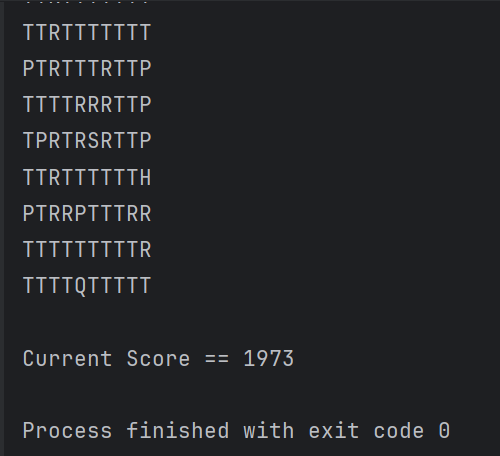
\includegraphics[width=\textwidth]{./images/score_simple}
	  		\caption{امتیاز محیط ساده}
	  		\label{fig:e}
	  	\end{subfigure}
	  	\hspace{0.5em}
	  	\begin{subfigure}{0.24\textwidth}
	  		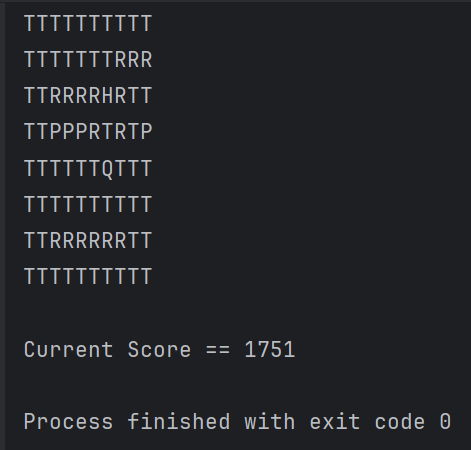
\includegraphics[width=\textwidth]{./images/score_hard}
	  		\caption{امتیاز محیط سخت}
	  		\label{fig:f}
	  	\end{subfigure}
	  	\hspace{0.5em}
	  	\begin{subfigure}{0.24\textwidth}
	  		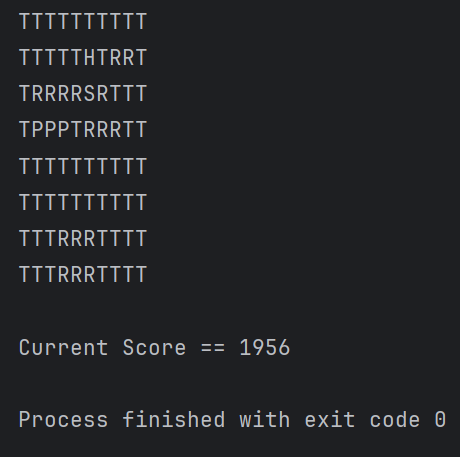
\includegraphics[width=\textwidth]{./images/score_t1}
	  		\caption{امتیاز محیط تست ۱}
	  		\label{fig:g}
	  	\end{subfigure}
	  	\hspace{0.5em}
	  	\begin{subfigure}{0.24\textwidth}
	  		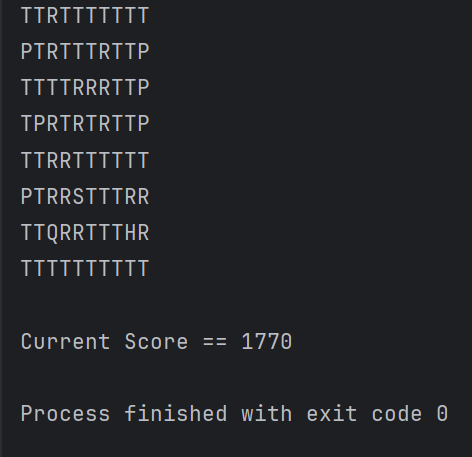
\includegraphics[width=\textwidth]{./images/score_t5}
	  		\caption{امتیاز محیط تست ۵}
	  		\label{fig:h}
	  	\end{subfigure}
	  	\caption{امتیازهای نهایی برای اجرای هر محیط}
	  	\label{scores}
	  \end{figure}
	  
	
	
	\section{بخش اختیاری}
	
	\subsection{مقدمه}
	هدف از اجرای این بخش کار کردن با یک محیط چند عاملی بود که نه تنها یک حریف رفتار خصمانه با ما دارد، ما هم چنین رفتاری نسبت به حریف داریم و هدف کسب بیشترین امتیاز در این محیط قطعی مشاهده‌پذیر کامل با ۳ عامل است.
	
	\subsection{پیاده‌سازی الگوریتم}
	برای چنین محیطی هدف این بود که ما یک الگوریتم جستجوی چند عاملی طراحی کنیم. برای این منظور، ما  یک تابع برای گرفتن بهترین اکشن داریم.
	
	از آنجا که کنش‌های ما پشت سر هم است، تابع گرفتن بهترین اکشن توسط ما برای بهینگی و پرهیز از اجرای تکراری یکبار اجرا می‌شود و دو اکشن می‌دهد که هر اکشن در موقع خود استفاده می‌شود. یعنی در مرتبه‌ای که اکشن پرنده صدا زده می‌شود، هیچ محاسبه‌ای انجام نمی‌شود و صرفا اکشن صحیح برمی‌گردد.
	
	سپس الگوریتم مینی ماکس به کمک هرس آلفا بتا روی تمام کنش‌های ممکن اجرا می‌شود و بهترین کنش‌ها برمی‌گردند و از آن برای انجام کنش استفاده می‌شود. 

نکته‌ی حائز اهمیت در اینجا این است که برای کنش پرنده و مرغ اگر حرکت به سمت دیوار یا خارج از محیط بازی انجام شود، اولا امتیازی کسر نمی‌شود (یعنی کنش محسوب نمی‌گردد) ثانیا باعث می‌شود که اندازه‌ی فاصله فرد یا زوج شود. به لحاظ تئوری برای رسیدن به هدف باید اندازه‌ی فاصله فرد باشد و اگر اندازه‌ی فاصله زوج باشد رسیدن به هدف ممکن نیست.

اگرچه ما از هرس آلفا بتا هم استفاده کردیم اما عمق جستجو به سختی می تواند عدد ۵ باشد. بهترین عملکرد را از لحاظ زمانی در عمق ۳ و ۴ داریم. شاید اگر از یک روش برای کش کردن حالت‌های تکراری استفاده می‌کردیم، بسیار الگوریتم کاراتری داشتیم.

\subsection{توابع هیوریستیک}
\subsubsection{هیوریستیک تخمین حالت انتهایی}
تابع هیوریستیک ما در اثنای پروژه مکررا تغییر پیدا کرد و موارد زیادی به آن اضافه و کم شدند. تابع هیوریستیک به ما کمک می‌کند در گریدهایی که محیط انتهایی بازی نیست، تخمینی از اینکه این حالت از بازی به چه امتیازی ختم می‌شود برسیم. 


ما تابع هیوریستیک را طوری طراحی کردیم که هیچ‌وقت امتیاز آن بیشتر از مقدار واقعی نشود. ما برای تعریف تابع هیوریستیک، از فاصله‌ی مرغ تا تخم مرغ‌ها، فاصله‌ی مرغ تا ملکه، فاصله‌ی پرنده تا ملکه، فاصله‌ی خوک‌ها تا مرغ، زوج بودن فاصله‌ی پرنده تا ملکه استفاده کردیم.
	\subsubsection{هیوریستیک مرغ}
	هیوریستیک مرغ هم همان هیوریستیک  حالت انتهایی است. البته در جایی هم امتیاز نهایی را به عنوان هیوریستیک در نظر گرفتیم. از آنجا که هدف هیوریستیک مرغ بیشنیه کردن حالت انتهایی است، مرغ هم با این هیوریستیک به خوبی کار می‌کند.
	
\subsubsection{هیوریستیک ملکه}
ما برای تخمین حالت بهینه برای خوک از یک تابع فاصله‌ی منهتنی ساده استفاده کردیم و دنباله‌های ممکن را بر اساس آن مرتب کردیم.

\subsubsection{هیوریستک پرنده}
ما دو وظیفه به پرنده محول کرده‌ایم. اول رسیدن به خوک و دومی جلوی خوک را گرفتن برای اینکه به سمت پرنده حرکت نکند. این مخصوصا در حالت hard زیاد اتفاق می‌افتد که پرنده جلوی حرکت خوک را بگیرد.

\end{document}